

% ****** Start of file aipsamp.tex ****m*
%
%   This file is part of the AIP files in the AIP distribution for REVTeX 4.
%   Version 4.1 of REVTeX, October 2009
%
%   Copyright (c) 2009 American Institute of Physics.
%
%   See the AIP README file for restrictions and more information.
%
% TeX'ing this file requires that you have AMS-LaTeX 2.0 installed
% as well as the rest of the prerequisites for REVTeX 4.1
% 
% It also requires running BibTeX. The commands are as follows:
%
%  1)  latex  aipsamp
%  2)  bibtex aipsamp
%  3)  latex  aipsamp
%  4)  latex  aipsamp
%
% Use this file as a source of example code for your aip document.
% Use the file aiptemplate.tex as a template for your document.
\documentclass[%
 aps, pra,
% jmp,
% bmf,
% sd,
% rsi,
 amsmath,amssymb,
%preprint,%
 preprint,%
%author-year,%
%author-numerical,%
% Conference Proceedings
superscriptaddress
]{revtex4-2}

\usepackage{graphicx}% Include figure files
%\usepackage{dcolumn}% Align table columns on decimal point
\usepackage{bm}% bold math
\usepackage{fixme}
%\usepackage[mathlines]{lineno}% Enable numbering of text and display math
%\linenumbers\relax % Commence numbering lines
\usepackage{hyperref}
\usepackage{kbordermatrix}% http://www.hss.caltech.edu/~kcb/TeX/kbordermatrix.sty
\usepackage[utf8]{inputenc}
\usepackage[T1]{fontenc}
\usepackage{mathptmx}
\usepackage{lipsum}
\usepackage{amsmath}
\usepackage{physics}
\usepackage{xparse}
\usepackage{bbm}
\usepackage{xcolor}
\usepackage{url}


%\usepackage{multirow}
%\usepackage{makecell}
\graphicspath{{Pictures/}}

\renewcommand*{\figureautorefname}{Fig.}
\renewcommand*{\equationautorefname}{Eq.}

\newcommand{\mytitile}{Supplementary matrials for Photon transport in a Bose-Hubbard chain of superconducting artificial atoms}

\begin{document}
	\preprint{AIP/123-QED}
	
	\title[\mytitile]{\mytitile\\~}
	
\maketitle


\section{Linear regime} \label{sec:app_linear}

In the linear regime with no pure dephasing, the Langevin equations for the steady state read:
\begin{equation}
\begin{aligned}
0 &= i(\omega_1 - \omega_d)\hat b_1^\dag - \frac{\gamma_1}{2} \hat b_1^\dag + i J\hat b_2^\dag + \sqrt{\gamma_1}b_{in}^\dag,\\
0 &= i(\omega_2 - \omega_d)\hat b_2^\dag - \frac{\gamma_2}{2} b_{2}^\dag + i J\hat b_{1}^\dag + i J\hat b_{3}^\dag,\\
0 &= i(\omega_3 - \omega_d)\hat b_3^\dag - \frac{\gamma_3}{2} \hat b_{3}^\dag + i J\hat b_{2}^\dag + i J\hat b_{4}^\dag,\\
0 &= i(\omega_4 - \omega_d)\hat b_4^\dag -\frac{\gamma_4}{2} \hat b_{4}^\dag + i J\hat b_{3}^\dag + i J\hat b_{5}^\dag,\\
0 &= i(\omega_5 - \omega_d)\hat b_5^\dag - \frac{\gamma_5}{2} \hat b_5^\dag + i J\hat b_4^\dag,
\end{aligned} 
\end{equation}
omitting zero-photon fluctuations. The solution of this system used for the model curves in Fig. 3~(a) of the main paper is too complex to display; however, for the degenerate case it becomes rather simple:
\begin{equation}
\hat b_{{5}}^\dag={\frac {4\,i{J}^{4}\sqrt {\Gamma} \hat b_{in}^\dag}{ \left( i\delta\,
\Gamma+2\,{\delta}^{2}-2\,{J}^{2} \right)  \left( i{\delta}^{2}
\Gamma-2\,i{J}^{2}\Gamma+2\,{\delta}^{3}-6\,\delta\,{J}^{2
} \right) }}.\label{eq:s21}
\end{equation}
Here, $\delta = \omega_d - \omega$. For the case of strong coupling, $J\gg \Gamma$, one can find that the poles of this expression are at $0, \pm J, \pm \sqrt 3 J $. This is a particular case of a more general statement considering the crystal dispersion relation: for a system of size $N$, the crystal momentum takes $N$ values $k = \frac{2 \pi}{N+1} m,\ m=\pm 1, \pm 2... m \leq N/2,\ m\in \mathbb{Z}\  \cup\ {0}$ if $ N $ is odd. Then the corresponding dispersion relation is $E/\hbar = \omega + 2 J \sin k/2$.

Using the Taylor expansion near each of the poles of \eqref{eq:s21}, one can express is in the Lorentzian form and extract its width in the limit of $J \gg \Gamma$. This procedure will lead to the values $\Gamma/6,\ \Gamma/2,\ 2\Gamma/3$ for the peaks at the detunings $\pm \sqrt{3 J},\ \pm J, 0$, respectively. The sum of the widths equals to $2\Gamma$ and is conserved even when the transmons are arbitrarily detuned from the resonance. 


\section{Two-qutrit analytical solution}
It is instructive to discuss also a simple model of a chain of two identical three-level transmons; this case can be solved analytically. However, even for a pair of qutrits the exact analytical expression for the steady state is too cumbersome work with. Therefore we suggest to analyze its series expansion with respect to the driving amplitude. In the leading order in $f$, the density matrix elements in the steady state can be represented as
$$
\rho_{\text{ss}} = \rho_{\text{ss}}^{ij|i'j'} \propto \sum_{i,j,i',j'} f^{i+j}\, \ket{i,j}\bra{i',j'}
$$
Here $i,\ i'$ correspond to the states of the first transmon and $j,\ j'$ of the second. We split all elements of the density matrix into groups according to its leading order $n$ in $f$. We start from the case $n=0$. In this group there is only single element related to the transmon's ground state, so for this element we have $\rho^{11|11}_{\text{ss}}=1$. As the next step, $n=1$, there are four linear equations for density matrix elements $\rho^{11|12}_{\text{ss}}$, $\rho^{11|21}_{\text{ss}}$, $\rho^{12|11}_{\text{ss}}$ and $\rho^{21|11}_{\text{ss}}$. Here we take into account the result at the previous step  $\rho^{11|11}_{\text{ss}}=1$. We continue this iterative procedure for $n=2, 3, \dots$ and find the remaining density matrix elements. Thus, we finally find the series expansion for 

$$
\sigma^-_{2}
=
\mathbbm{1} \otimes \begin{pmatrix}
0 & 0 & 0
\\
\sqrt{2}& 0 & 0
\\
0 & 1 & 0
\end{pmatrix}
$$
as
\begin{gather*}
\langle\sigma_{2}^- \rangle
=\,
\text{Tr}\left [ \sigma_{2}  \rho_{\rm ss}\right]
=
\rho^{11|21}_{\rm ss}
+
\rho^{22|21}_{\rm ss}
+
\rho^{33|21}_{\rm ss}
+
\sqrt{2} \left(
\rho^{11|32}_{\rm ss}
+
\rho^{22|21}_{\rm ss}
+
\rho^{33|21}_{\rm ss}
\right)
=\\
-
\frac{16 \Omega J}{16 J^2 + (\Gamma - 4 i \delta)^2}
\\
-\frac{4096 \Omega^3 J^3 (\alpha -i \Gamma -4 \delta )}{(2 \alpha -i \Gamma \
	-4 \delta ) \left(16 J^2+(\Gamma -4 i \delta )^2\right) \left(16 \
	J^2+(\Gamma +4 i \delta )^2\right) \left(16 J^2+(\Gamma -4 i \delta ) \
	(2 i \alpha +\Gamma -4 i \delta )\right)}\\
\vdots
\end{gather*}
where $\delta = \omega_d - \omega$ is the detuning. We stress that in this expansion each element is calculated in its leading order with respect to $\Omega$. For the sake of simplicity, we consider the case $\Gamma \to 0$. In this limit, the term linear in $\Omega$ has two poles $\delta = \pm J$ which we attribute to single-photon resonances. The third order term has three additional poles $\delta = \alpha/2$, $\delta =(\alpha \pm \sqrt{16 J^2 + \alpha^2})/4$ which can be attributed to the two-photon processes. In the fifth order there will be additional three-photon pole at
$\delta = (\alpha \pm 2J)/3$. The result of the numerical calculation of $\langle\sigma_{2}^-\rangle$ for different $\Omega$ and $\omega$ is represented in Fig. \ref{fig:map-sminus-2qb3-log}. As one can see, with the increase of driving power, when driving power become of order of damping, dips appear at frequencies we have determined. This feature is expectable for multi-photonic processes and it is due to effective inverse occupation of the third transmon levels. It occurs when the occupancy of the transmon third level exceeds a second level occupancy, that results in effective suppression of a single-photon process.

\begin{figure}
	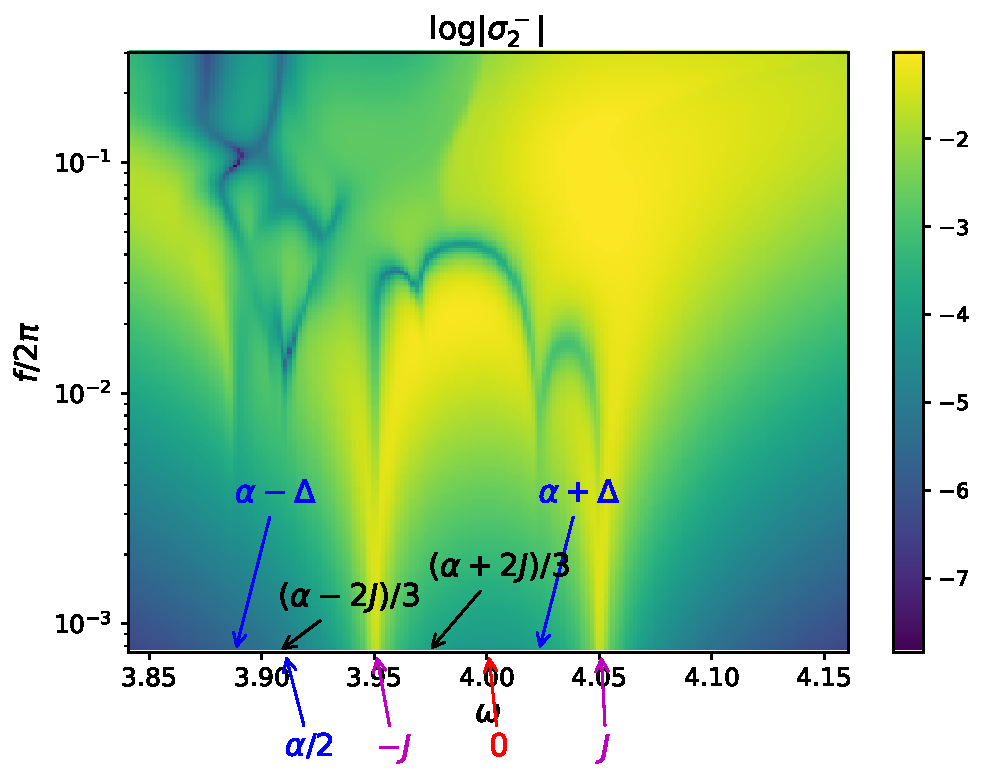
\includegraphics[width=0.7\linewidth]{Pictures/map-sminus-2qb3-log.pdf}
	\caption{Analytical solution using the expansion of the density matrix. Arrows denote the identified transitions, where $\Delta = \sqrt{16 J^2 + \alpha^2}$, $\omega/2\pi = 4$ GHz, $\alpha/\pi = -181$ MHz, $J/2\pi = 50$ MHz, $\gamma \approx 3.2\, \mu\text{s}^{-1}$.}
	\label{fig:map-sminus-2qb3-log}
\end{figure}


There is another approach to find the resonant frequencies responsible for multiphoton processes. 
the Hamiltonian in the rotating frame does not depend on time explicitly. In addition it conserves excitation number, $N$, so it can be split into independent sectors with particular $N$ which we denote as $H_{(N)}$.
In each sector we find eigenenergies:
\begin{widetext}
$$
\begin{array}{ccc}
H_{(1)} = \begin{pmatrix}
-\delta & J
\\
J & -\delta
\end{pmatrix},
\qquad &
\delta = \pm J;
\\[1em]
H_{(2)} = \begin{pmatrix}
\alpha - 2\delta & \sqrt{2} J & 0
\\
\sqrt{2} J & - 2\delta & \sqrt{2} J
\\
0 & \sqrt{2} J & \alpha - 2 \delta
\end{pmatrix},
\qquad &
\displaystyle
\delta = \frac{\alpha \pm \sqrt{16 J^2 + \alpha^2}}{4}, \quad \delta = \frac{\alpha}{2};
\\[2em]
H_{(3)} = \begin{pmatrix}
\alpha - 3\delta & 2J
\\
2 J & \alpha - 3 \delta
\end{pmatrix},
\qquad & \displaystyle
\delta = \frac{\alpha \pm 2 J}{3};
\\[2em]
H_{(4)} = \begin{pmatrix}
2 \alpha - 4\delta
\end{pmatrix},
\qquad & \displaystyle
\delta = \frac{\alpha}{2}.
\end{array}
$$
\end{widetext}
This result illustrates why there is no specific poles in series expansion of $\langle\sigma_{2}^-\rangle$ in seventh order: four-photon process is hidden by a two-photon process since both of them have the same energy. This accidental coincidence is a feature of this particular configuration with a couple of three-level systems. For example, if we treat transmons as  four-level systems, then this effect will not occur and four-photon process will be distinguishable.







\end{document}